\chapter{Integrating NoSQL in the Virtual Observatory}

Modern relational databases have shown little efficiency in certain applications using intensive data, like indexing of a large number of documents, sites rendering with high traffic, and streaming sites.

Typical RDBMS implementations are tuned either for small but frequent reads and writes or a large set of transactions that have few write accesses. On the other hand, NoSQL DB are optimized for read and bulk-ingest operations, and perform outstandingly where a relational DB would slow down. They are especially fast when large amounts of data have to be queried, and if we consider that speed is more important than consistency\footnote{Consistency is used here in the sense of having changes replicated to multiple nodes at the same time. RDBMS ensure that consistency, but that makes them less performat. Given that VO users do not know beforehand whether some datasets are available or not, speed in data retrieval and operations is more important than consistency (which will not be perceived unless for special circumstances).}.

As mentioned in the chapter on the Virtual Observatory, the
IVOA has a standard called Astronomical Data Query Language (ADQL) that users do not necessarily need to know, because
they % users is 3-rd person plural
can pose a query with a GUI, as long as the query is translated into standard ADQL. The receiving service likewise converts the standard ADQL into whatever its own database servers need, but always inside
the
relational model. For the reasons stated in Chapter~\ref{theproblem}, we propose the use of a different approach, the NoSQL technology.


\section{Introduction to NoSQL} % (fold)
\label{sec:nosql}

A non-relational database just stores data without explicit and structured mechanisms to link data from different buckets to one another.

NoSQL implementations used in the real world include 3TB Digg
social media website\urlnote{http://digg.com}
green markers (indicated to highlight the stories voted by others in the social network), the 6 TB of
the ENSEMBLES\urlnote{http://ensemble2.jrc.ec.europa.eu/public/}
European Commission
Joint Research Centre (JRC)
database used in comparing models and air quality, and the 50 TB of Facebook inbox search. 

NoSQL architectures often provide limited consistency, such as events or transactional consistency restricted to only data items. Some systems, however, provide all guarantees offered by
% ACID systems
systems compliying with the Atomicity, Consistency, Isolation and Durability (ACID) criteria
by adding an intermediate layer.
The ACID properties guarantee the reliable processing of database transactions, but they are not needed for system where the data are not subject to transactions, such as read-only systems.

There are two systems that have been deployed and provide for storage of snapshot isolation column: Google Percolator (based on BigTable system) and Hbase transactional system developed by the University of Waterloo. These systems use similar concepts in order to achieve distributed multiple rows ACID transactions with snapshot isolation guarantees for the underlying storage system in that column,
with % typo: wit
no extra overhead in data management, no system deployment middleware or any maintenance introduced by middleware layer. 

Many % quite
NoSQL systems employ a distributed architecture, maintaining data redundantly on multiple servers, often using distributed hash tables. Thus, the system may actually escale adding more servers, and thus a server failure may be tolerated. 

There are different NoSQL DBs for different projects:

\begin{description} % {itemize}

\item[Document oriented] These are systems whose main purpose is to record document data and metadata, such as text corpuses, massive mail systems, or similar datasets.

  \begin{itemize}
    \item CouchDB\urlnote{http://couchdb.apache.org}
    \item MongoDB\urlnote{http://www.mongodb.org}
    \item RavenDB\urlnote{http://ravendb.net}
    \item IBM Lotus Domino\urlnote{http://www.ibm.com/software/products/us/en/ibmdomino/}
  \end{itemize}

\item[Graph oriented] These are systems whose emphasis is made in recording the relationships (including directionality) between the objects in the data store.

  \begin{itemize}
    \item Neo4j\urlnote{http://www.neo4j.org}
    \item AllegroGraph\urlnote{http://www.franz.com/agraph/allegrograph/}
    \item InfiniteGraph\urlnote{http://www.objectivity.com/infinitegraph}
    \item Sones GraphDB\urlnote{https://github.com/sones/sones}
    \item HyperGraphDB\urlnote{http://www.hypergraphdb.org/}
  \end{itemize}

\item[Key-value oriented] These are systems where simple key-value pairs (such as those in FITS headers) are stored, withing a shallow hierarchy of metadata.

% NOTA: Añadir \urlnote para el resto de los sitemas

  \begin{itemize}
    \item Cassandra\urlnote{http://cassandra.apache.org/}
    \item BigTable\urlnote{http://research.google.com/archive/bigtable.html}
    \item Dynamo (Amazon)\urlnote{http://aws.amazon.com/dynamodb/}
    \item MongoDB\urlnote{http://www.mongodb.org/}
    \item Project Voldemort (LinkedIn)\urlnote{http://www.project-voldemort.com/voldemort/}
  \end{itemize}

\item Multivalue

  \begin{itemize}
    \item OpenQM\urlnote{http://www.openqm.com/cgi/lbscgi.exe?t0=h&t1=home}
  \end{itemize}  

\item[Object Oriented] These systems try to store complex objects, their metadata and relationships in ways that are directly usable by software systems to save and retrieve internal state.
  
  \begin{itemize}
    \item Zope Object Database \urlnote{http://www.zodb.org/en/latest/}
    \item db4o\urlnote{http://www.db4o.com/}
    \item GemStone S\urlnote{http://gemtalksystems.com/index.php/products/gemstones/}
    \item Objectivity/DB\urlnote{http://www.objectivity.com/}
  \end{itemize}

\item[Tabular] These systems provide support for storing very large tables, but not for relationships between them.

  \begin{itemize}
    \item HBase\urlnote{http://hbase.apache.org/}
    \item BigTable
    \item LevelDB (BigTable open version)\urlnote{http://code.google.com/p/leveldb/}
    \item Hypertable\urlnote{http://hypertable.org/}
  \end{itemize}
\end{description} % \end{itemize}

All of these systems can % They
run on clusters of inexpensive machines,
or can be run on distributed cloud systems such as the Amazon Elastic Cloud, Google App Engine, or similar.

% section nosql (end)


\section{Advantages and uncertainties of NoSQL} % (fold)
\label{sec:advantages_and_uncertainties_of_nosql}

\begin{description} % {itemize}

\item[Elastic scaling] % \textbf{Elastic scaling}

DBA have relied on scale up — buying bigger servers as database load increases — rather than scale out — distributing the database across multiple hosts as load increases. However, as transaction rates and availability requirements increase, and as databases move into the cloud or onto virtualized environments, the economic advantages of scaling out on commodity hardware become irresistible.

Unlike RDBMS, the NoSQL databases are designed to expand transparently to scale and they are usually designed with low-cost in mind.


\item[Economics] % \textbf{Economics}

NoSQL databases typically use cheap clusters servers, while RDBMS tends to rely on expensive proprietary servers and storage systems. The result is a lower cost per transaction/second for NoSQL.


\item[Flexible data models] % \textbf{Flexible data models}

Even minor changes to the data model of an RDBMS have to be carefully managed and may necessitate downtime or reduced service levels. NoSQL databases have a less strict (in the worst case) data model restrictions. NoSQL allows the application to store virtually any structure it wants in a data element. The result is that application changes and database schema changes do not have to be managed as one unit. In theory, this will allow applications
and user facing services
to iterate faster.

\item[No need for DBAs] % \textbf{No need for DBAs}

% Este argumento me da un poco de miedo. Cuidado cuando hagas la exposición, o con las preguntas que puedan hacer.

RDBMS systems can be maintained only with the assistance of expensive and highly trained DBAs, while NoSQL databases are generally designed to require less management:  automatic repair, data distribution, and simpler data models lead to lower administration and tuning requirements and costs.

\end{description} % \end{itemize}


NoSQL systems have generated a lot of enthusiasm, but there are still a lot of questions about its future:

\begin{description} % {itemize}

\item[Maturity] % \textbf{Maturity}

RDBMS systems have been around for a long time. NoSQL evangelists will argue that their advancing age is a sign of their obsolescence, but mature RDBMS systems are stable. Most NoSQL alternatives are in pre-production versions with many key features yet to be implemented.

\item[Support] % \textbf{Support}

Most NoSQL systems are open source projects, and although there are usually one or more firms offering support for each NoSQL database, these companies often are small start-ups.
There are risks in chosing a NoSQL solution that is no longer supported in the future, but at the same time, if the community is large enough, NoSQL systems can maintain their deployability for longer time.

\item[Expertise] % \textbf{Expertise}

There are millions of developers with expertise using RDBMS. On
the % ther
other hand, NoSQL developers are, by far, a minority. This situation seems to
be changing, % change,
but for now, it is easier to find experienced RDBMS programmers or
DBAs % DBA
than NoSQL experts.

\end{description} % \end{itemize}

% section advantages_and_uncertainties_of_nosql (end)

\section{NoSQL deployments in scientific research} % (fold)
\label{sec:nosql_deployments_in_scientific_research}

To support our proposal of implementing
NoSQL systems in the VO, % a NoSQL system,
we present in this
subsection
some successful case studies which show that selecting such a new alternative (in comparison with the classical RDBMS) 
for big scientific projects is
not necessarily % more than
a risk, the main reason argued
against NoSQL. % by NoSQL detractors.

\subsection{CMS at the LHC: MongoDB} % (fold)
\label{sub:cms_at_the_lhc_mongodb}
High-energy physicists working at the Compact Muon Solenoid (CMS) detector at the LHC, that generates more than 100 datacentres in a three-tier model and generates around 10PB of data each year, are benefiting from a NoSQL database management system that gives them unified access to data from a huge variety of sources (from relational and non-relational data sources, such as relational databases, document-oriented databases, blogs, wikis, file systems and customised applications). The team providing data management to the CMS Cern project has built a system using MongoDB in preference to relational database technologies and other non-relational options. The reasons to select MongoDB were:

\begin{itemize}
\item Dynamic queries support
\item Full indexes
\item Auto-sharding
\end{itemize}

Several years ago the data management group at the CMS confronted a data discovery problem, with a variety of databases necessitating a user interface that would hide the complexity of the underlying architecture from the physicists. There was a vast variety of distributed databases and different formats (HTML, XML, JSON files, etc.).

To provide the ability to search and aggregate information across this complex data landscape CMS's Data Management and Workflow Management (DMWM) project created a
Data Aggregation System (DAS),
built on
top of
MongoDB.  According to Valentin Kuznetsov, a research associate at Cornell University, and team member, \emph{``there was nothing specific to the system related to our experiment''}\urlnote{http://www.computerweekly.com/news/2240166469/Cornell-Cern-project-plumps-for-NoSQL-DBMS}, so it can be deduced that this MongoDB approach is extensible.
% NOTA: Añadir link o publicación como cita del entrecomillado

% subsection cms_at_the_lhc_mongodb (end)

\subsection{ATLAS Workload Management System: Cassandra} % (fold)
\label{sub:atlas_workload_management_system_cassandra}

A Thoroidal LHC Apparatus (ATLAS) is another of the six particle detectors experiments
at LHC % at LHC at CERN,
whose data handling is a real challenge: almost 1 billion
proton-proton
interactions per second
are recorded,
leading to more than 10PBytes per year (it actually generates 1PByte of raw data each second, before filtering). By 2014, the expected data rate will be 40 PBytes per year.

% \begin{figure}[tb]
% \centering
% 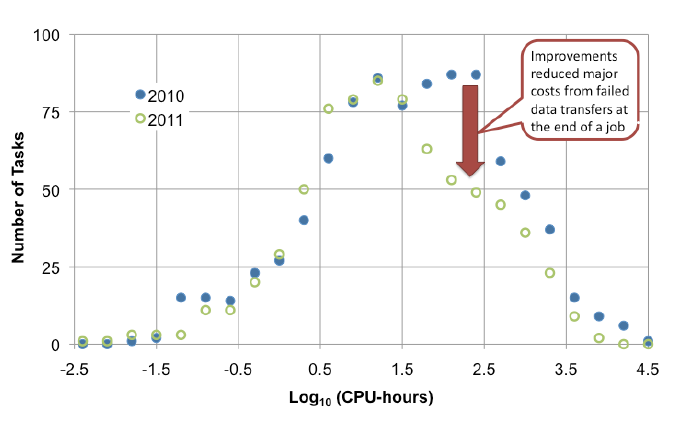
\includegraphics[width=14cm,height=8cm]{images/panda.png}
% \caption{Weibull distribution of CPU-hours used to recover job failures in petascale data processing, from \href{https://sharepoint.anl.gov/hep/HEP\%20Accomplishments/Highlights_101212.pdf}{Argonne National Laboratory}}
% \end{figure}

The reason to select a NoSQL solution is
that
there is no need to store the monitoring data in a RDBMS, deciding instead a system which can provide a very high degrees of availability, resilience and scalability.

At first stage, two of the most popular platforms were considered: Apache
Cassandra\urlnote{http://cassandra.apache.org/}
and Apache Hbase\urlnote{http://hbase.apache.org}.
% As

Cassandra was finally selected, as its learning curve is less steep % Cassandra has a lower learning curve, 
and for ease of operation.\urlnote{http://cds.cern.ch/record/1446655/files/ATL-SOFT-PROC-2012-012.pdf}
and considering that
there was % it was
already
a Cassandra deployment within the ATLAS collaboration,
% deployed in ATLAS, the decision was done. % NOTA: Estaría bien saber por qué Cassandra se usaba ya en ATLAS.
the solution was taken.

As a matter of fact, in the tests
performed, % done,
Cassandra's time per extracted entry was 10 ms, with 10 concurrent clients. This means 1000 queries per second, about twice the rate currently experienced by their Oracle DB. An analogous test done against Oracle (from a Python client) yielded roughly 100ms per
query\footnote{See \url{http://cds.cern.ch/record/1446655/files/ATL-SOFT-PROC-2012-012.pdf}}.

% subsection atlas_workload_management_system_cassandra (end)

\subsection{Measuring radiation levels in Seattle: CouchDB} % (fold)
\label{sec:measuring_radiation_levels_in_seattle_couchdb}

Researchers at the University of Washington used the Cloudant \urlnote{https://cloudant.com/} database as part of an experiment that determined radiation levels in Seattle as a result of the recent Fukushima nuclear disaster are \emph{``well below alarming limits.''}\urlnote{http://gigaom.com/2011/03/31/how-nosql-is-helping-allay-seattles-radiation-fears/} The research team, which includes Cloudant Founder and Chief Scientist Mike Miller studied particles captured from the five air filters and used Cloudant’s CouchDB-based BigCouch database to store and process the data.

They chose Cloudant because with it, it was possible to start monitoring radiation levels very quickly, after a very easy setup and the capability of sampling gigantic quantities of air, allowing them to analyze the data and sharing it in near-real-time,
benefiting from BigCouch's MapReduce engine.

% NOTA: Añadir link o publicación como cita del entrecomillado
% NOTA: Mejorar, si es posible, este último párrafo de justificación

% subsection measuring_radiation_levels_in_seattle_couchdb (end)


% section nosql_deployments_in_scientific_research (end)

% \section{MongoDB: a document oriented database} % (fold)
\section{Choosing a NoSQL database: MongoDB} % (fold)
\label{sec:mongodb_a_document_oriented_database}

MongoDB (from \emph{humongous}) is an open source document-oriented
NoSQL
database system developed and supported by 10gen.
% It is part of the NoSQL family of database systems.
Instead of storing data in tables as is done in a \emph{classical} relational database, MongoDB stores structured data as JSON-like documents with dynamic schemas (MongoDB calls the format BSON), making the integration of data in certain types of applications easier and faster. 

An example of Mongo DB document insertion is shown in Listing~\ref{lst:docinsert}.

\begin{lstlisting}[float,label=lst:docinsert,caption=MongoDB column insertion example in JSON]
db.columns.insert( {
		table_name: "TAP_SCHEMA.schemas",
		column_name: "schema_name",
		utype: null,
		ucd: null,
		unit: null,
		description: "schema name for reference to TAP_SCHEMA.schemas",
		datatype: "VARCHAR",
		size: 64,
		principal: 1,
		indexed: 0,
		std: 0
	}
);
\end{lstlisting} 


10gen began Development of MongoDB in October 2007 and was not created to be just another database that tries to do everything for everyone. Instead, MongoDB was created to work with documents rather than rows, was extremely fast, massively scalable, and easy to use. In order to accomplish this, some
RDBMS
features were excluded, namely
the
support for transactions.

%\begin{shaded}
A document database is more like a collection of documents. Each entry is a document, and each one can have its own structure. If you want to add a field to an entry, you can do so without affecting any other entry.
%\end{shaded} 



% \subsection{Why MongoDB?}
\subsection{Justification} % (fold)
\label{sub:justification}

We have decided to use MongoDB for these reasons:

\begin{itemize}
\item It is open source code (available at \url{https://github.com/mongodb/mongo}).
\item It is widely used in the NoSQL community.
\item It has full index %support
support, which is a must for large datasets
\item It is very
easy to install and to connect through drivers with several programming languages like Java, Python, Ruby, C/C++, PHP or Scala.
\item It supports
the
MapReduce paradigm.
\item It is possible to connect MongoDB with Hadoop (the \emph{de facto} big data processing and analytics platform \urlnote{http://hadoop.apache.org},
allowing to to send MongoDB data into Hadoop MapReduce jobs, process the data and return it back to a MongoDB collection).
\end{itemize}

The following subsection provices a more detailed list of MongoDB features.

% subsection justification (end)

\subsection{Main features} % (fold)
\label{sub:main_features}

\begin{description} % {itemize}

\item[Ad-hoc queries] % \textbf{Ad hoc queries} 
MongoDB supports search by field, range queries, regular expression searches. Queries can return specific fields of documents and also include user-defined JavaScript functions.

\item[Indexing] % \textbf{Indexing} 
Any field in a MongoDB document can be indexed (indices in MongoDB are conceptually similar to those in RDBMS).

\item[Data replication] % \textbf{Replication} 
MongoDB supports master-slave replication. A master can perform reads and writes. A slave copies data from the master and can only be used for reads or backup (not writes). The slaves have the ability to select a new master if the current one goes down.

\item[Load balancing] % \textbf{Load balancing} 
MongoDB scales horizontally using sharding (a shard is a master with one or more slaves). The developer chooses a shard key, which determines how the data in a collection will be
distributed\footnote{For instance, astronomical collections can be naturally split in different sky stripes, object types, magnitude ranges, et cetera.}. % distributed.
The data is split into ranges (based on the shard key) and distributed across multiple shards. MongoDB can run over multiple servers, balancing the load and/or duplicating data to keep the system up and running in case of hardware failure. Automatic configuration is easy to deploy and new machines can be added to a running database.

\item[File storage capabilities] % \textbf{File storage} 

MongoDB could be used as a file system, taking advantage of load balancing and data replication features over multiple machines for storing files. This feature, GridFS, is included with MongoDB drivers and available for development languages. GridFS is used, for instance, in plugins for NGINX and lighttpd. In a multi-machine MongoDB system, files can be distributed and copied multiple times between machines transparently, thus effectively creating a load balanced and
fault-tolerant % fault tolerant
system.

\item[Aggregation] % \textbf{Aggregation} 
MapReduce can be used for batch processing of data and aggregation operations. The aggregation framework enables users to obtain the same results as the SQL
\texttt{GROUP BY}
clause.

\end{description} % \end{itemize}

Once we have seen the main features of MongoDB, we can move on to the 
system % language
itself~\cite{MongoWeb,Chodorow10,Chodorow11}.

% subsection main_features (end)


% \subsection{The basics}
\subsection{MongoDB concepts} % (fold)
\label{sub:mongodb_concepts}

We must know four concepts to understand MongoDB: Database, Collection, Document, and Field. The correspondence between the document-oriented MongoDB terminology, and that of relational systems is shown in
Table~\ref{tab:relationalvsdocument}

% dig into MongoDB's world:

% \begin{description} % {itemize}
% \item[Database] this concept is much like the RDBM counterpart.
% \item[Collection] we can see a collection and a table as the same thing.
% \item[Document] its equivalent in
% a RDBMS % RDBM
% is the 
% row; % row, and
% a document is made up of fields.
% \item[Field] it is equivalent to a column % is a lot like a column.
% \end{description} % \end{itemize}


\begin{table}
\begin{center}
\begin{tabular}{ll} % NOTA: no se deben usar línas verticales en tablas
% \hline
\textbf{Relational} & \textbf{Document oriented} \\ \midrule[2pt]
Table & Collection\\ \midrule % \hline
Row & Document\\ \midrule % \hline
Column & Field \\
% \hline
\end{tabular}
\end{center}
\caption{Correspondence between relational and NoSQL terminology}
\label{tab:relationalvsdocument}
\end{table}



% \begin{figure}[tb]
% \centering
% 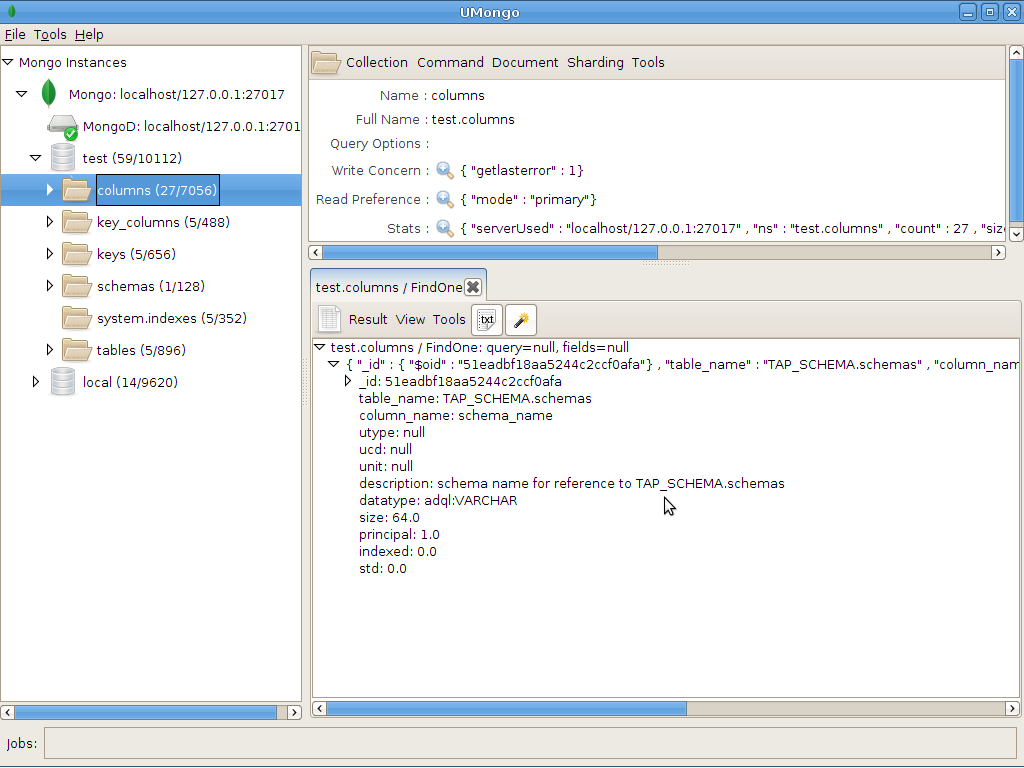
\includegraphics[width=11cm,height=8cm]{images/mongo_dia.png}
% \caption{Tree View for Tap Schema in MongoVue}
% \end{figure}


\subsubsection{SQL/Mongo syntax differences}

In this subsection we can see some differences in the DDL syntax used by both SQL and MongoDB. For the latter, we can call it from any language having a driver to connect to the DB or use the interactive shell (the code presented here uses this shell). Listing~\ref{lst:sqlvsmongo} shows the differences in syntax between the DDL instructions for SQL and MongoDB.

\lstinputlisting[float,language=SQL,caption={Syntax comparison between SQL and MongoDB BSON for table/document creation, document/row insertion, document/row selection, document/row deletion, and document/row updates.},label=lst:sqlvsmongo]{src/sample01.sql}

% subsection mongodb_concepts (end)

\subsection{MongoDB MapReduce support} % (fold)
\label{sub:mongodb_mapreduce_support}

\begin{figure}[tb]
\centering
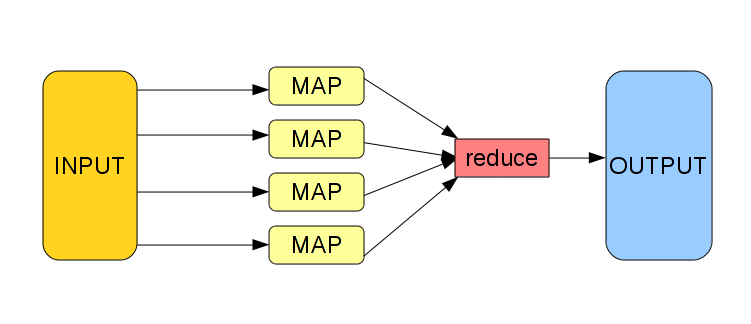
\includegraphics[width=\textwidth]{images/map_reduce_chart.png}
\caption{MapReduce concept}
\label{fig:mapreduce}
\end{figure}

MapReduce, developed by Google, is a programming model and its implementation for processing (\textit{e.g.} raw data from telescopes) and producing (\textit{e. g.} representations of graph structure of systems) huge amounts of data. As the runtime controls the partitioning of the input data, controlling the program execution across several hundred or thousands of nodes and even controlling machine failures, the developers with low or none expertise at all in parallel programming can take advantage of this model with a very low learning curve.
The concept is illustrated in Fig.~\ref{fig:mapreduce}.

MapReduce
is usually used % usually, is used
to solve problems involving big size datasets, up to several petabytes. For this reason, this model is used in distributed file systems, like
the Hadoop Distributed File System (HDFS)\urlnote{http://hadoop.apache.org/docs/stable/hdfs_design.html}.

The MapReduce model allows to write a \emph{map} function which takes a key/value pair, operates on it
(for instance, performs FITS-file multi-header and/or multi-table calculations)
and returns a new set of key/value pairs
(source list of FITS files with values above a given threshold). % (source list).
The \emph{reduce} function then aggregates/merges all the intermediate data (builds an object catalog removing duplicates from the source list, for instance).
% Many problems in astronomy naturally fall into this model because of the inherent parallelizability of many astronomical tasks.

Problems in different domains can be parallelized via MapReduce, by a suitable definition of both the \emph{map} and \emph{reduce} functions. In particular, tasks whose only changes are the input values can be \emph{map}ped to the input arguments and output arguments, and the \emph{reduce} function can be a trivial sumation of null outputs from the \emph{map} functions, while the important result has been saved by the \emph{map}ped function (in a save-file, for instance).


Listing~\ref{lst:mapreducesample} shows how to define a MapReduce job in MongoDB.

\lstinputlisting[float,label=lst:mapreducesample,language=Java,caption=MapReduce job example]{src/map_reduce_01.js}

% subsection mongodb_mapreduce_support (end)


% section mongodb_a_document_oriented_database (end)

% \section{Creating FITS alternative in MongoDB}
\section{Creating a FITS store in MongoDB} % (fold)
\label{sec:creating_a_fits_store_in_mongodb}

The first issue when working with FITS files is its inadequacy for storing information. In XXI century is difficult to maintain such storage model. So the first and more obvious solution would be replacing FITS headers with their counterparts in a non relational database. 

Another issue when working with FITS format is the great amount of possible key-value pairs in FITS headers. A possible solution for this problem could be use the features of MongoDB to translate FITS keywords into collections. So, we could create as
many % much
documents as needed, and storing them into MongoDB. Should we need to create supertypes of FITS headers, relations are also available in MongoDB through document linking (with no physical restriction in the sense of relational constraint). In this situation the schema flexibility means that we can model documents that share a similar structure but not enforced to have to same.

Another related problem is having multiple FITS formats\footnote{The IAU FITS Working Group (IAU-FWG) is the international control authority for the FITS (Flexible Image Transport System) data format: \url{http://fits.gsfc.nasa.gov/iaufwg/iaufwg.html}}, representing the users need for storing and handling the different information requirements:

\begin{itemize}
\item FITS Interferometry Data Interchange (FITS-IDI) Convention: conventions adopted for registering information from interferometric telescopes recordings. Used by the VLBA.
\item Single Dish FITS (SDFITS) Convention for Radio Astronomy Data: conventions used for the interchange of single dish data in radio astronomy. 
\item Multi-Beam FITS Raw Data Format Convention: conventions used at the IRAM 30m and APEX 12m mm/submm telescopes.
\item OIFITS: A Data Standard for Optical Interferometry Data: conventions used for exchanging calibrated, time-averaged data from astronomical optical interferometers.
\end{itemize}


We show now a logical layout using MongoDB features to solve the previously posed problem. Let's suppose we have several FITS files and we have to handle them as easy as possible.

For the sake of simplicity and clarity, we have not included all FITS keywords, focusing on the abstraction.

Several proposals
for storing
FITS
header metadata
in a database have been made. One of the examples is the ESO 
Keyword Repository~\cite{2008SPIE.7016E..51V}, a metadata database containing all information stored in almost 10 million FITS file headers using Sybase IQ server\urlnote{http://www.sybase.com/products/datawarehousing/sybaseiq}, a columnar storage RDBMS.

For this work, we can profit from MongoDB document-oriented storage support (collections, documents and fields). MongoDB allows to define as
many % much
kinds of documents as needed, sort of meta-documents, considering that there is no compulsory for them having the same structure. 

\paragraph{Solution}

Using just one collection and $n$ documents, one for each kind. If we are going to work with FITS-IDI, SDFITS, MBFITS and OIFITS, we can use code like to create different variations of what a FITS document is like.

We start from a very simple FITS header like: 

\begin{lstlisting}[float,label=lst:fitsheader,caption=FITS sample.]
SIMPLE = T / Standard FITS format
BITPIX = 8 /
NAXIS = 0 /
EXTEND = T /
BLOCKED = T /
OBJECT = 'BINARYTB' /
TELESCOP= 'VLBA ' /
CORELAT = 'VLBA ' / added to header dump by EWG
FXCORVER= '4.22 ' /
OBSERVER= 'BL146 ' /
ORIGIN = 'VLBA Correlator' /
DATE-OBS= '2007-08-23' /
DATE-MAP= '2007-08-31' / Correlation date
GROUPS = T /
GCOUNT = 0 /
PCOUNT = 0 /
END
\end{lstlisting}

Prior to translating it into MongoDB, we create several collections in Listing~\ref{lst:fitstypes}, one for each different FITS types.

\begin{lstlisting}[float,label=lst:fitstypes,caption=MongoDB BSON code for creating the different FITS document types.]

db.fits_type.insert(
  {convention: "FITS-IDI"}
);

db.fits_type.insert(
  {convention: "SDFITS"}
);

db.fits_type.insert(
  {convention: "MBFITS"}
);

db.fits_type.insert(
  {convention: "OIFITS"}
);

\end{lstlisting}


Now, inserting the primary HDU for a  FITS-IDI header in MongoDB could not be
easier, given the fact that FITS headers are collections of key-value pairs. % easier.

This code is very easy to translate into MongoDB syntax, as shown in Listing~\ref{lst:fitsinsert}.

\begin{lstlisting}[float,label=lst:fitsinsert,caption=MongoDB BSON code for adding FITS metadata to the NoSQL database.]

db.fits_docs.insert(
    {convention: "FITS-IDI",
    SIMPLE: "T",
    BITPIX: 8,
    NAXIS: 0,
    EXTEND: "T",
    BLOCKED: "T",
    OBJECT: "BINARYTB",
    TELESCOP: "VLBA ",
    CORELAT: "VLBA ",
    FXCORVER: "4.22 ",
    OBSERVER: "BL146 ",
    ORIGIN: "VLBA Correlator",
    DATE_OBS: "2007-08-23",
    DATE_MAP: "2007-08-31",
    GROUPS: "T",
    GCOUNT: 0,
    PCOUNT: 0}
);

\end{lstlisting}

Note that we have specified a field named \emph{supertype}, which acts as a foreign key in a RDMS. This field help to classify FITS files, despite MongoDB collections do not enforce the structure of its documents.

Now, we have our FITS header into a database with a document structure. We keep the same approach but in a very more usable and efficient way.

% section creating_a_fits_store_in_mongodb (end)



% \section{Rewriting ALMA Science Archive}
\section{Scaling the ALMA Science Archive: Bridging OpenCADC and NoSQL} % (fold)
\label{sec:rewriting_the_alma_science_archive_with_nosql}
 
As stated in~\cite{2009ASPC..404..324E}, the purpose of the ALMA archive is to provide services for:

\begin{itemize}

\item Persistent archiving and retrieval for observational data.

\item Search and retrieval of observations via several descriptors. % Observaction descriptors.

\item Retrieval of reduced datacubes
% Datacubes
produced by
the
pipeline.

\item Search and retrieval of technical and environmental data. % Technical and environmental data.
\end{itemize}

The main objective of the
ALMA Archive
conceptual design (see Fig.~\ref{fig:asa_afa})
is to guarantee that three ALMA Regional Centres (North America,
East Asia % Japan
and Europe) hold an identical copy of the archive at the Joint ALMA Observatory in Santiago. 

The ALMA Front-end Archive (AFA; the part of the archive directly accessed by the ALMA correlator)
is optimized for storage and preservation, not for data query and retrieval.

The ALMA Science Archive (ASA), on the other hand, is the user-facing part of the ALMA Archive, the interface for querying ALMA data. The ASA receives a transformed copy of the data from the AFA, because only a subset of the data and metadata in the AFA is considered to be queriable by the users.

\begin{figure}
\centering
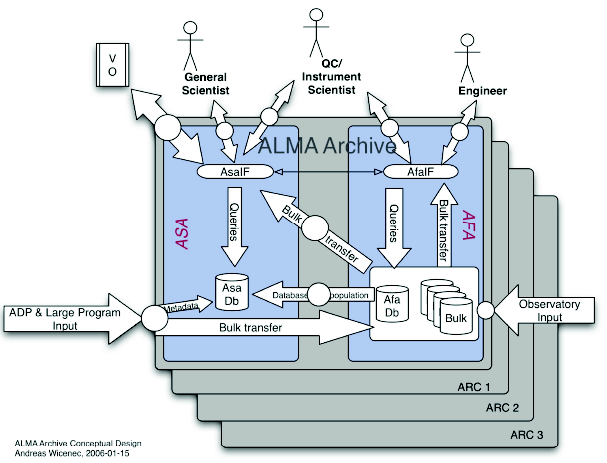
\includegraphics[width=0.8\textwidth]{images/alma_science_archive.png}
\caption{ALMA Science Archive and ALMA Front-end Archive; figure by A. Wicenec.}
\label{fig:asa_afa}
\end{figure}


% NOTA: desconectado del resto de la explicación
% ASA database is inspired from ObsCore, RADAMS and Hubble Legacy Archive plus Virtual Observatory Software:
% \begin{itemize}
% \item openCADC (\ref{sec:opencadc}), which is used for database access and VO access protocol
% \item VOView, for Web components
% \end{itemize}

% TODO: Incluir 


Despite all ALMA information can be accessed from the Archive, ASA provide a optimized way to access the data in a scientific way. One of the requirements of ASA design was to provide a search and query tool which allows several parameters (position, frequency, telescope related parameters, etc.). It has two major components: the DB, which is a plain relational database with denormalized structure and the interface
(shown in Fig.~\ref{fig:asaqueryif}),
built as a web application.

\begin{figure}
\centering
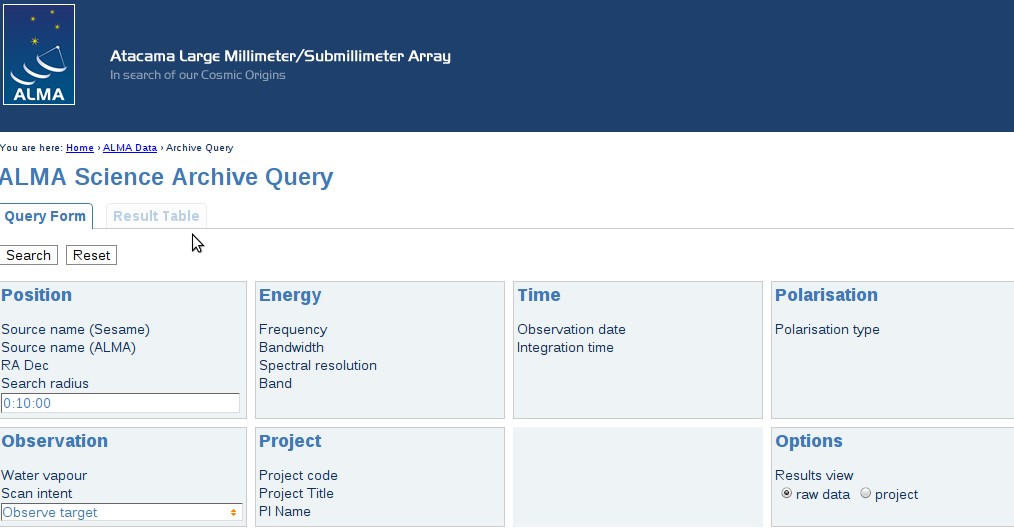
\includegraphics[width=\textwidth]{images/aq.png}
\caption{ALMA Science Archive Query Interface}
\label{fig:asaqueryif}
\end{figure}

\begin{figure}
\centering
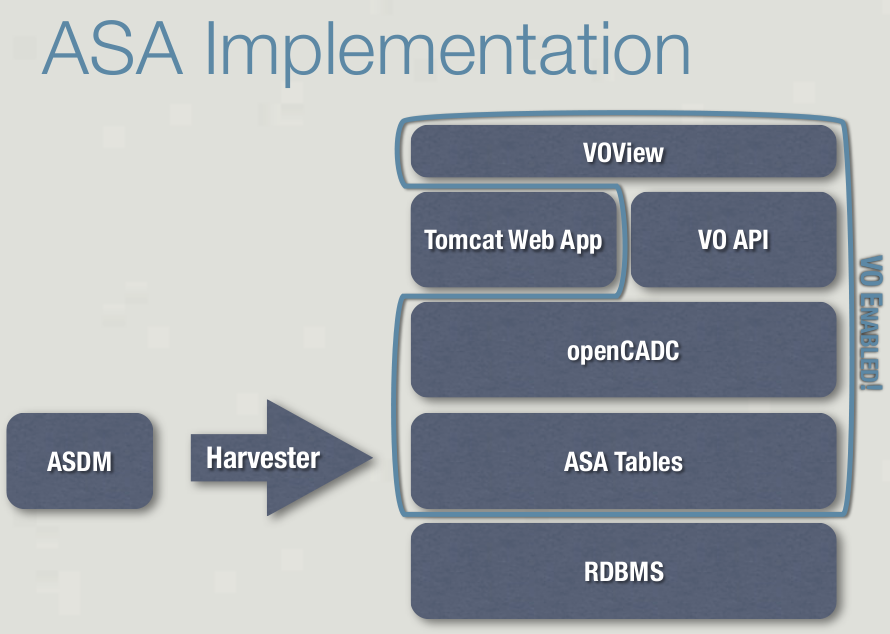
\includegraphics[height=8cm]{images/asa_implementation.png}
\caption{ALMA implementation diagram, courtesy of   \href{http://amiga.iaa.es/FCKeditor/UserFiles/File/VOandALMAarchive_web.pdf}{Juande Santander}}
\label{fig:asa_implementation}
\end{figure}


The VO Technologies used in the ALMA Archive are (discussed in Chapter~\ref{cha:the_virtual_observatory}):

\begin{enumerate}
\item VO Data Models
\item Software libraries
  \begin{enumerate}
    \item OpenCADC
    \item VOView\urlnote{http://code.google.com/p/voview/}: a JQuery-based JavaScript component for viewing large data tables within a Web browser, reformatting XML VOTables into HTML in the browser.
  \end{enumerate}
\end{enumerate}



\subsubsection{OpenCADC-MongoDB Interface}


After studying NoSQL DBMS and showing their pros, in this section we assume we want to rewrite the Web application from ASA shown in Fig.~\ref{fig:asa_implementation} to use a non-relational DBMS like MongoDB.

To take advantage of the existing OpenCADC work, our proposal is to use MongoDB and Java programming language.

We connect Java and MongoDB using two methods:

\begin{enumerate}

\item The MongoDB-provided Java driver \urlnote{http://docs.mongodb.org/ecosystem/drivers/java/}

\item The Spring framework\urlnote{http://www.springsource.org}, a comprehensive programming and configuration model for Java-based enterprise applications. The Spring Data MongoDB \urlnote{http://www.springsource.org/spring-data/mongodb} provides an extension to the Spring programming model that support writing applications for the new datastores, like MongoDB or CouchDB database. There is no need to use any additional component, provided we have this software.

\end{enumerate}

We have chosen the second option, as Spring Data framework reduces notably the amount of code to be written. Let's see a comparison between the traditional Mongo way and the Spring Data one in Listing~\ref{lst:classic_new}.

% NOTA: No se explica qué hace esto
\begin{lstlisting}[float,label=lst:classic_new,caption=Old vs new syntax Mongo-Java connection.]
// The classic MONGODB-JAVA connection
public List<cols> getAll() {
  
  logger.debug("Retrieving all columns data");

  DBCollection coll = MongoDBFactory.getCollection("asa_db","coll_tables");
  DBCursor cur = coll.find();
  List<cols> items = new ArrayList<cols>();

  while(cur.hasNext()) {
    DBObject dbObject = cur.next();
    Cols cols = new Cols();

    cols.setColumnName(dbObject.get("Column_name").toString());
    cols.setTableName(dbObject.get("Table_name").toString());
    cols.setTableUcd(dbObject.get("Ucd").toString());
    cols.setTableUtype(dbObject.get("Utype").toString());
    
    ... // omitting the rest of fields

    items.add(cols);
  }

  return items;

}


// New implementation with Spring Data
public List<Cols> getAll() {

  logger.debug("Retrieving all columns data");

  Query query = new Query(where("pid").exists(true));
  List<Cols> cols = mongoTemplate.find(query, Cols.class);

  return cols;

}
\end{lstlisting}

To accomplish this job, we have identified three major stages:

\paragraph*{Defining a MongoDB schema for ObsCore}
\label{sec:mongodb_obscore}
To support the use cases identified in ObsCore IVOA documentation \urlnote{http://www.ivoa.net/documents/ObsCore/20110502/PR-ObsCore-v1.0-20110502.pdf} we must identify a set of elements that any ObsTAP service must support, ensuring that any query based on these parameters is guaranteed to be understood by all ObsTAP services.
The ObsCore model must be implemented within TAP services, so that all queries can be executed, without changes have to be made, on any service that implements the model.
\texttt{TAP\_SCHEMA} is the database schema where the tables and columns exposed by the service are described.



\paragraph*{Addressing the data input}
\label{sec:data_input}
We have previously commented in Section~\ref{sec:creating_a_fits_store_in_mongodb} the model used to solve the problems that arise when publishing archives with FITS (and their particular metadata to standard models that in some cases need to be completed with metadata not available in FITS headers) files to the VO.

\paragraph*{Adapting the existing Java code}
\label{sec:spring_mongo}